\documentclass[11pt]{article}
\usepackage{textcomp}
\usepackage{longtable}
\usepackage{graphicx}
\usepackage{subcaption}
\usepackage{listings}
\usepackage{color}
\usepackage{paralist}
\usepackage[hyphens]{url}
\usepackage{geometry}
\usepackage{wrapfig}

% \usepackage{titlesec}
% \newcommand{\sectionbreak}{\clearpage}

\geometry{a4paper, left=25mm, top=25mm}

\definecolor{codegreen}{rgb}{0,0.6,0}
\definecolor{codegray}{rgb}{0.5,0.5,0.5}
\definecolor{codepurple}{rgb}{0.58,0,0.82}
\definecolor{backcolour}{rgb}{0.95,0.95,0.92}

\lstdefinestyle{mystyle}{
    backgroundcolor=\color{backcolour},
    commentstyle=\color{codegreen},
    keywordstyle=\color{magenta},
    numberstyle=\tiny\color{codegray},
    stringstyle=\color{codepurple},
    basicstyle=\footnotesize,
    breakatwhitespace=false,
    breaklines=true,
    captionpos=b,
    keepspaces=true,
    numbers=left,
    numbersep=5pt,
    showspaces=false,
    showstringspaces=false,
    showtabs=false,
    tabsize=2
}

\lstset{basicstyle=\footnotesize,style=mystyle}

\linespread{1.29}

\graphicspath{ {Images/}{Graphs/} }
\author{Eugene Valetsky\\ \and Supervisor: Dr Tim Baker}
\title{Unmanned Aerial Systems}

%%%%%%%%%%%%%%%%%%%%%%%%%%%%%%%%%%%%%%%%%%%%%%%%%%%%%%%%%%%%%%%%%%%%%%%%%%%%%%%
% DOCUMENT
%%%%%%%%%%%%%%%%%%%%%%%%%%%%%%%%%%%%%%%%%%%%%%%%%%%%%%%%%%%%%%%%%%%%%%%%%%%%%%%
\begin{document}
\maketitle

\begin{center}
    GitHub Repository: \url{https://github.com/eugeneval/Project_Titan}

    \vspace{2em}
    Word Count: 7314


    \vspace{6em}
    \emph{I, Eugene Valetsky, confirm that the work presented in this report is my own. Where information has been derived from other sources, I confirm that this has been indicated in the report.}
\end{center}

\newpage
\tableofcontents
\listoffigures
\newpage



\section{Abstract}
The goal of this project is to design and test, in a simulated environment, the control system for a vehicle to compete in the Institution of Mechanical Engineers (\emph{IMechE}) Unmanned Aerial Systems (\emph{UAS}) Challenge. This vehicle must be capable of autonomous flight, which will include GPS waypoint navigation, location of a ground target, and the accurate delivery onto a payload onto said target\cite{IMechE_rules}.

\subsection*{Design Concept Validation}
The UAS design uses a novel concept: a traditional quadcopter built around a central micro jet engine\cite{Ismail_paper}. This is an as-yet untested configuration and investigation was required to ensure it was controllable. Equations of motion were derived from first principles for a simplified model of the airframe, and a computer simulation was built in Processing\cite{processing} to test the feasibility of the chosen configuration, especially with regards to the impact that the jet engine would have on stability. Results showed that while stability was significantly impacted over a pure quadcopter, especially in height, it was still within acceptable margins.

\subsection*{Control System Design}
A control system was designed consisting of a PixHawk flight controller running the PX4 software\cite{PX4_user_guide}, augmented by a companion computer running custom-made software to handle the duties of control, communication, and computer vision. Python\cite{python} was chosen as a programming language due to its simplicity, abundance of available relevant libraries, and good cross-platform compatibility.

The three main modules for the companion computer software were built and tested: control of the PixHawk, communication with a ground station, and target-finding computer vision.
These were tested using a software-in-the-loop (\emph{SITL}) PX4 simulation and the jMAVSim simulation environment. The DroneKit SDK was used as the basis for control of the PixHawk, but it had to be modified, as it was originally designed to work with APM, the predecessor of PX4\cite{dronekit}. Commands for connecting to the PX4, taking off, navigating it both using GPS coordinates and in the local frame of reference, navigating it using both absolute and relative coordinates, and returning to base were all created and tested thoroughly within the simulation environment of jAVSim. Computer vision is done using the OpenCV-Python library. The target is recognised by searching for concentric squares in the image. Optical Character Recognition (\emph{OCR}) is possible using the Tesseract and pytesseract libraries. Communication will be by radio, and so will be limited to a serial connection. Functions were created and tested which allowed the transfer of crucial information, such as the coordinates of a located target, over said serial connection using the JSON format.

These separate modules were brought together, and allow a simulated drone to navigate to a target, by using the offset of the target from the center of the frame as an input for a command navigating to a target relative to the current position. A specific companion computer was chosen, the Raspberry Pi3. The control system was ported to the companion computer, and modifications were made to account for the details of running on specific hardware.

\subsection*{Conclusion}
The airframe concept has been validated in a simulated environment and stability has been shown to be within acceptable margins. Control software has been designed, created, and tested in a simulated environment. The control system is ready for deployment to the real vehicle as and when it is complete.


\section{Introduction}
The Unmanned Aerial System (UAS) Challenge was launched by the Institution of Mechanical Engineers (IMechE) in 2014 `with the key objectives of developing professional engineers and inspiring the next generation'\cite{IMechE_about_uas}. The main goal is to design and build a UAS in order to autonomously deliver humanitarian aid such as medical supplies in a disaster zone. This requires a broad range of skills, from project management to airframe design to avionics system programming. To add to the challenge there is a strict weight limit and stringent safety regulations. Working together with another student, Ismail Ahmad, our goal is to follow the design and build cycle all the way through to competing at the IMechE UAS competition in June 2018.

One of the greatest individual challenges as part of the project is creating an autonomous flight system. The UAS must be capable of quickly and safely navigating to and locating a target using computer vision, dropping a payload accurately, and returning to base. This requires an understanding of the UAS’s flight dynamics as well as good programming and wiring capabilities. This is the aspect that I will be focusing on for my individual project. I will also be assisting with other parts of the project, but this is outside the scope of this report.


\subsection{Airframe Design}
The concept for our UAS uses a hybrid symbiosis between a \emph{Micro Jet Engine}, henceforth referred to as MJE, and an external multi-rotor. The MJE is gimballed to always remain vertical and only provides lift, while the multi-rotor rotates around it providing stabilisation and control. This configuration means that standard quadcopter flight control software can be used rather than needing to come up with custom architecture.

The MJE provides a higher thrust to weight ratio than the equivalent electric motors and batteries. It does this without introducing the vibration issues of a piston engine, which would seriously impact stability and control on such a lightweight design. With the current MJE and electric motors we hope to lift a payload of 3kg while remaining under the 6.9kg weight limit imposed by the rules\cite{IMechE_rules}. MJE's are also capable of running on a wide variety of fuels, which would be an advantage in a disaster zone where fuel and electricity supplies may be limited or unavailable\cite{Ismail_paper}.

The chosen airframe configuration is a novel airframe that, to the extent of research done into the subject, has only been tried by several hobbyists and never as a serious technical endeavour. We were to discover only quite late in the design process (see Section \ref{payload_delivery}) a possible reason as to why - the central MJE greatly complicates the carriage of payload.

Further detail as to the physical design of the airframe is outside the scope of this project, as this is Ismail Ahmad's responsibility\cite{Ismail_paper}. A render of his design for the airframe can be seen in Figure \ref{fig:saucy_render}\cite{Ismail_paper}.

\begin{figure}[h]
    \begin{subfigure}{0.48\textwidth}
        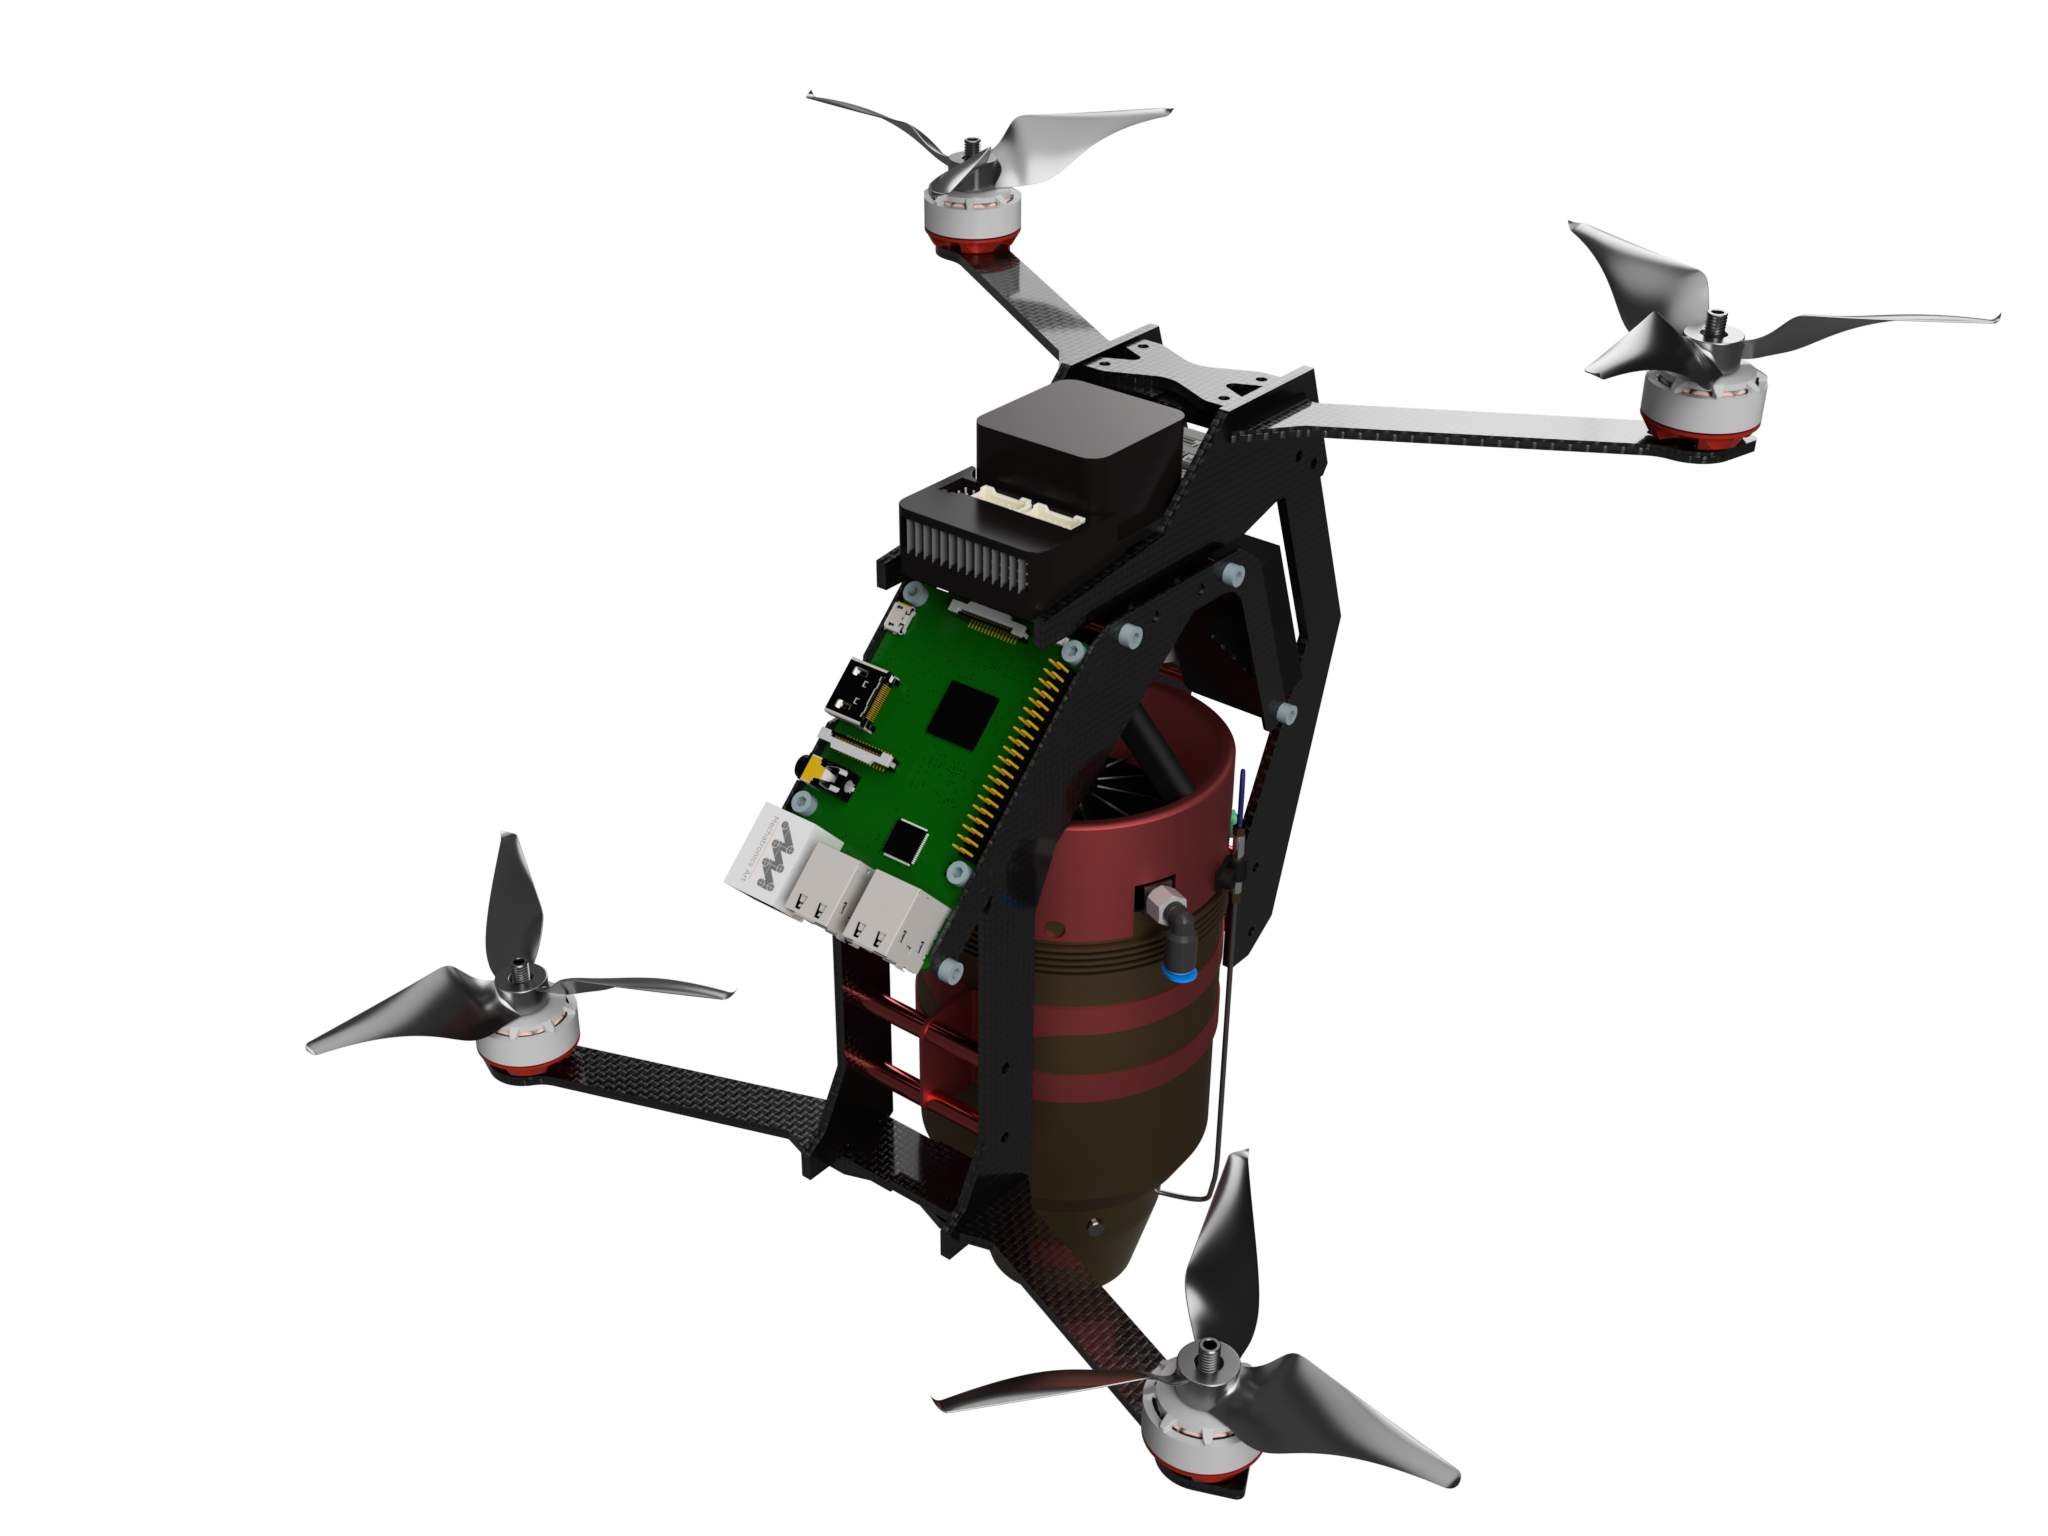
\includegraphics[width=\linewidth]{saucy_render_bare}
        \caption{Bare}
        \label{fig:saucy_render_bare}
    \end{subfigure}\hspace*{\fill}
    \begin{subfigure}{0.48\textwidth}
        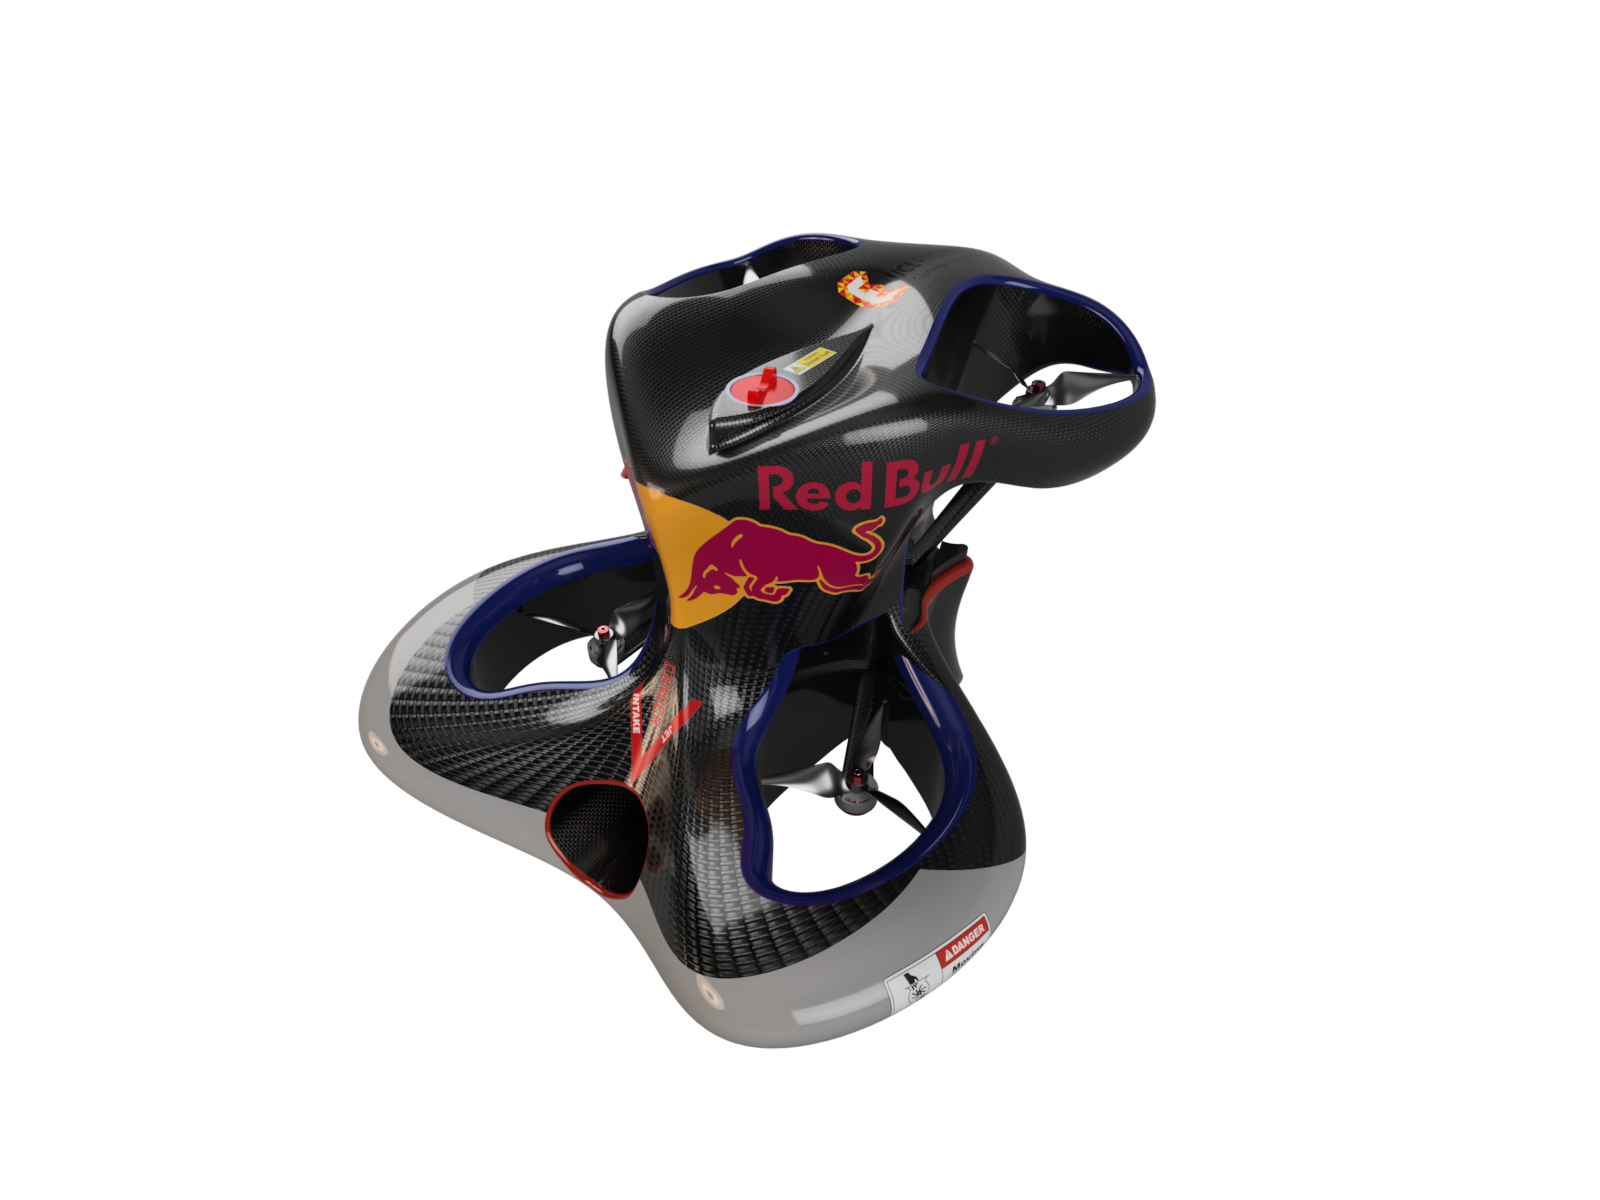
\includegraphics[width=\linewidth]{saucy_render_w_bodyshell}
        \caption{With Bodyshell}
        \label{fig:saucy_render_w_bodyshell}
    \end{subfigure}

    \caption{Renders of Airframe Design}
    \label{fig:saucy_render}
\end{figure}


\subsection{Aim and Objectives}
Ultimately, the long term goal of this project is to take part in the IMechE UAS Challenge. However, within the extent of the third-year project, the objectives are as follows:

\begin{compactenum}
    \item Determine, via simulation or otherwise, whether the stability of the airframe configuration is within acceptable parameters.
    \item Investigate and design a control system for the UAS. This control system must be able to:
    \begin{compactenum}
        \item Travel to predetermined GPS waypoints.
        \item Recognise and navigate to a target using computer vision.
        \item Communicate the GPS coordinate of the target to a ground station.
    \end{compactenum}
    \item Test the control system in a simulated environment.
\end{compactenum}


As this is an open-ended design project, the exact details of the final solution cannot be determined at this stage. The nature of the design process for a new vehicle means that precise details of the individual stages of the projects is not known at the start of the project.
As such, these aims and objectives have been expanded on in more detail in the relevant sections after initial research and design has been undertaken.

\subsection{Control System Design}
Flight control will be handled with a PixHawk running the PX4 flight stack. This will be coupled to a companion computer running software based on the DroneKit SDK, communicating with the PixHawk using the MAVLink protocol. The companion computer is responsible for communication, waypoint navigation, and target location and tracking using computer vision. It then communicates where to go to the PixHawk. This is not a new method of quadcopter flight control; rather, it is an adaption of existing software and methods to our specific airframe and the requirements of the UAS Challenge.

This setup of two computers working in tandem, a low-level flight controller and a high-level companion computer, is the currently widely accepted method for adding complex autonomy to small unmanned aerial vehicles\cite{student_drone_platform}. Computer vision is a computationally intensive task; we do not want it to 'distract' the flight controller from actually flying the vehicle, as flight control might be running at refresh rates of up to 50 times a second. The separation of flight control ensures the stability and reliability of the vehicle.

As the MJE is both expensive (\~\pounds1300), and fragile, it was decided to go for a top of the range flight controller in an effort to avoid costly crashes. Two main options were considered - the DJI A4 and the PixHawk 2. These are both considered excellent quality flight controllers, and also both allows for external control with a companion computer, using either the DJI SDK for the A4 or one of DroneCore, DroneKit, or MAVROS for the PixHawk. In the end, the PixHawk was chosen as it is open source, allowing for easier modification to our needs; there is also more documentation, tutorials, and other information available online for it.

Reasons for the choice of the DroneKit SDK over alternatives are explained in Section \ref{PX4 Control}. Companion computer selection is covered in Section \ref{cc_selection}. The full code can be found on GitHub at \url{https://github.com/eugeneval/Project_Titan}.


\section{Simulation of System Plausibility} \label{simulation}
\subsection{Concept}
One of the main concepts behind the UAS concept is the idea that, if the MJE is gimballed to remain vertical, and its thrust vector is through the center of gravity of the vehicle, it exerts no horizontal forces or moments on the rest of the vehicle. This means its effect on the stability and control of the vehicle can be ignored. In turn, this means that regular quadcopter flight control software can be used, such as the PX4 flight stack.

Being able to use PX4 firmware running on a PixHawk is crucial. The UAS will come to cost approximately \pounds2,500. Using home-made flight control software is therefore extremely risky. PX4, on the other hand, is a project that has been worked on by thousands of people for years, and is infinitely more reliable than anything we could put together from scratch. Additionally, creating custom flight control software is both discouraged by the IMechE, who recommend adapting an off-the-shelf autopilot \cite{IMechE_rules}, and falls well outside the scope of a university third-year project.

Therefore, it was decided to build a simulation to test the validity of the concept that the MJE can be ignored.

\subsection{Aims \& Objectives} \label{simulation objectives}
The specific objectives of this section of the project are:
\begin{compactenum}
    \item Create a simplified model of the airframe, consisting of easy to model shapes such as cylinders and cuboids.
    \item Derive equations of motion for this simplified model, describing how it will respond to forces, moments, and torques.
    \item Design a PID control system for the airframe
    \item Design and create a simulation environment incorporating this model, equations of motion, and controller, which will follow a test flight path and output relevant values to be analysed.
    \item Test the model as a quadcopter only (not including the MJE).
    \item Test the model with the MJE included.
    \item Decide, based on results of the simulation, whether the stability of the airframe configuration is within acceptable parameters.
\end{compactenum}

\subsection{Equations of Motion}
\begin{wrapfigure}{r}{0.5\textwidth}
    \begin{center}
        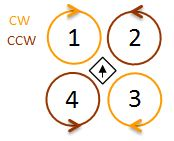
\includegraphics[width=0.48\linewidth]{Quad-X}
        \caption{Quadcopter Configuration}
        \label{fig:quad-x}
    \end{center}
\end{wrapfigure}
The vehicle is split into two sections, the outer quadcopter frame, \emph{Quad}, and the gimballed section containing the MJE, \emph{Jet}. A cartesian reference frame was chosen, with the xy plane being the horizontal plane and z being height. +x is right, +y is forward, +z is up. A rotation about the x axis is pitch, about the y axis is roll, and about the z axis is yaw. These are labelled $\theta_x, \theta_y,$ and $\theta_z$ for the quad and $\phi_x, \phi_y,$ and $\phi_z$ for the jet respectively.

The gimbal is controlled by two servos, one moving the gimbal in roll and one in pitch. (There is no need for yaw control of the jet.)  Note that this means $\theta_z = \phi_z$.

The multi-rotor uses the `quad-x' configuration, as shown in Figure \ref{fig:quad-x}. Note that motors 1 and 3 spin clockwise, and motors 2 and 4 spin anticlockwise. In the quad-x configuration, pairs of motors control each of the flight axes. For example, to pitch forward, motors 1 and 2 are spun down, and motors 3 and 4 are spun up; to yaw left, motors 2 and 4 would be spun up whilst motors 1 and 3 are spun down. The flight control system combines these various control movements, as well as ensuring that the net upward thrust is maintained. This can be seen in Equations \ref{eqn:FM1} through \ref{eqn:FM4}.


\subsubsection{Forces}\label{sec:Forces}
Our gimbal design will transmit forces, but not moments. Thus, from a forces perspective, the vehicle is treated as a single unit.

The quad is modelled as an inner thin, hollow cylinder, the \emph{frame}, with four cylindrical rods, the \emph{arms}, extending outwards. The motors are point masses on the ends of the arms. It is assumed to be constructed of aircraft-grade aluminium. The total mass is therefore:
\begin{equation}
    M_{TOT} = \underbrace{\rho\pi h (r_2-r_1)}_{Frame} + 4\cdot\underbrace{\rho\pi L r_r^2}_{Arms} + 4\cdot\underbrace{M_M}_{Motors} + 2\cdot\underbrace{M_G}_{Servos} + \underbrace{M_J}_{Jet} \label{eqn:total_mass}
\end{equation}
The forces acting on the system are:
\begin{eqnarray}
    F_x = (F_{M1} + F_{M2} + F_{M3} + F_{M4})\cdot\sin{\theta_x}\cdot\cos{\theta_z} +  F_J\cdot\sin{\phi_x}\cdot\cos{\phi_z} \\
    F_y = (F_{M1} + F_{M2} + F_{M3} + F_{M4})\cdot\sin{\theta_y}\cdot\cos{\theta_z} +  F_J\cdot\sin{\phi_y}\cdot\cos{\phi_z} \\
    F_z = (F_{M1} + F_{M2} + F_{M3} + F_{M4})\cdot\cos{\theta_x}\cdot\cos{\theta_y} +  F_J\cdot\cos{\phi_x}\cdot\cos{\phi_y}
\end{eqnarray}

\subsubsection{Quad Rotation}
With the quad design as described in Section \ref{sec:Forces}, the following inertias about the three defined axes are as follows:
\begin{eqnarray}
    I_{Qx} = I_{Qy} & = & \underbrace{\frac{\pi \rho h_F}{12}(3(r_2^4-r_1^4) + h_F^2(r_2^2-r_1^2))}_{Frame} \nonumber \\ & + & 4 \cdot \underbrace{\sin 45 \cdot (\frac{M_R L_R^2}{12}+M_R(r_2+\frac{L_R}{2})^2)}_{Arms} \nonumber \\ & + & 4 \cdot \underbrace{\sin 45 \cdot M_M(r_2+L)^2}_{Motors} \\
    I_{Qz} & = & \underbrace{\frac{\pi \rho h_F}{2}(r_2^4-r_1^4)}_{Frame} \nonumber \\ & + & 4 \cdot \underbrace{\frac{M_RL_R^2}{12} + M_R(r_2+\frac{L_R}{2})^2}_{Rods} \nonumber \\ & + & 4 \cdot \underbrace{M_M(r_2+L)^2}_{Motors}
\end{eqnarray}

On the quad, the gimbal servos exert offset moments about the z-axis. This results in the following equations:
\begin{eqnarray}
    \tau_{Qx} = (-F_{M1} - F_{M2} + F_{M3} + F_{M4})\cdot(L_R + r_2)\cdot \cos{45} \\
    \tau_{Qy} = (F_{M1} - F_{M2} - F_{M3} + F_{M4})\cdot(L_R + r_2)\cdot \cos{45} \\
    \tau_{Qz} = (F_{M1} - F_{M2} + F_{M3} - F_{M4})\cdot(L_R + r_2)\cdot \cos{45} + \tau_{Gx}\cdot r_1 + \tau_{Gy}\cdot r_1
\end{eqnarray}

\subsubsection{Jet Rotation}
Since $\theta_z = \phi_z$, we are only interested in the rotation of the jet about the x and y axes. Since there is a rigid linkage between the servo and the gimbal, the position of the servo is proportional to the rotation of the jet.

The jet is modelled as a cylinder. However, it does not rotate about its origin in x and y, but about the appropriate servo. Including the inertia of the servos themselves, calculated in Section \ref{servo_info} results in the following inertias:
\begin{equation}
    I_{Jx} = I_{Jy} = 3.89\times10^{-4} + M_J\cdot3r_J^2 + h_J^2 + M_Jl_c^2
\end{equation}

It can be seen in Section \ref{servo_info} the maximum torque the servo can exert is 0.34 kg-m. The actual torque exerted is controlled by a PID controller in order to keep the jet vertical.

\subsubsection{Servo Information}  \label{servo_info}
Servo information was based on a sample servo that may well end up being used on the vehicle, the Futaba BLS177SV.

\begin{center}
\begin{tabular}{ccc}
    Torque (at 6.6V): & 34 kg-cm \\
    Speed (at 6.6V): & 0.12sec/60\textdegree{} \\
    Weight: & 79g \\
\end{tabular}
\end{center}

We can see from the datasheet that it takes the servo 0.12 seconds to rotate 60\textdegree{}. Assuming it takes 0.01 of those seconds to accelerate to full speed, this gives an acceleration of $873rad/s^2$. Since we know it exerts a torque of 0.34kgm, this means its inertia must be $3.89\times10^{-4}$.

\subsection{PID Control} \label{sec:PID_Control}
8 PID controllers are needed in total: 3 position and 3 angle controllers for the quad, and 2 angle controllers for the jet gimbal. These controllers use the standard PID control logic:
\begin{eqnarray*}
    error = setpoint - actual\ value \\
    integral = integral + (error \times time\ period) \\
    derivative = (error - previous\ error)/time \\
    output = kP \times error + kI \times integral + kD \times derivative
\end{eqnarray*}
where kP, kI, and kD are constants to be optimised.

\subsubsection{Quad Control}
In a real quadcopter, the controller sends a signal to an \emph{electronic speed control} (ESC), which in turn sends a \emph{pulse width modulation} (PWM) signal to the motor, controlling its speed. In this model this has been simplified, such that the controller output directly controls the force exerted by the motors.

\begin{center}
\begin{tabular}{cc}
    $SP_x$ & Quad X position controller setpoint \\
    $SP_y$ & Quad Y position controller setpoint \\
    $SP_z$ & Quad Z position controller setpoint \\
    $SP_{\theta_x}$ & Quad X angle controller setpoint \\
    $SP_{\theta_y}$ & Quad Y angle controller setpoint \\
    $SP_{\theta_z}$ & Quad Z angle controller setpoint \\
    $O_x$ & Quad X position controller output \\
    $O_y$ & Quad Y position controller output \\
    $O_z$ & Quad Z position controller output \\
    $O_{\theta_x}$ & Quad X angle controller output \\
    $O_{\theta_y}$ & Quad Y angle controller output \\
    $O_{\theta_z}$ & Quad Z angle controller output \\
\end{tabular}
\end{center}

The controllers work in sequence, with the x and y position controllers determining the setpoint of the x and y angle controllers. The Z axis controller is independent.
\begin{eqnarray}
     O_x = SP_{\theta_x} \nonumber \\
     O_y = SP_{\theta_y} \nonumber \\
     F_{M1} = O_z - O_{\theta_x} + O_{\theta_y} + O_{\theta_z} \label{eqn:FM1} \\
     F_{M2} = O_z - O_{\theta_x} - O_{\theta_y} - O_{\theta_z} \\
     F_{M3} = O_z + O_{\theta_x} - O_{\theta_y} + O_{\theta_z} \\
     F_{M4} = O_z + O_{\theta_x} + O_{\theta_y} - O_{\theta_z} \label{eqn:FM4}
\end{eqnarray}

\subsubsection{Jet Gimbal Control}
Servos are controlled by sending an electronic signal to tell them what position to rotate to.

\begin{center}
\begin{tabular}{cc}
    $SP_{\phi_x}$ & Jet X angle controller setpoint \\
    $SP_{\phi_y}$ & Jet Y angle controller setpoint \\
    $O_{\phi_x}$ & Jet X angle controller output \\
    $O_{\phi_y}$ & Jet Y angle controller output \\
\end{tabular}

\begin{eqnarray}
    \tau_{Jx} = O_{\phi x} \\
    \tau_{Jy} = O_{\phi y}
\end{eqnarray}
\end{center}

\subsection{Programming}
The simulation itself was written in Processing. This is a language originally based on Java that is designed for ease of programming, especially with regards to displaying graphical elements\cite{processing}. It was chosen over using MATLAB due to the author's increased familiarity with it, and the fact that this simulation has no need of advanced mathematical capability - there are no complex differential equations or matrix operations. Previous simulations of quadcopters have generally used Newton-Euler equations\cite{quad_modelling_matlab}\cite{quad_modelling}, but these have been deliberately avoided in this model.

The program was built up in stages, with the physics of each stage checked before adding complexity. As far as possible, good object-oriented programming practice has been followed.

The quad section was implemented first. A controller was first tested solely in the z direction, and the response was used to calibrate PID values for the z controller. Angular controllers were then implemented, tested, and calibrated, before finally introducing x and y position controllers.

Testing involved flying a simple path: takeoff to 10m, a square path (10m north, 10m east, 10m south, 10m west), and then landing. This gave the results seen in Figure \ref{fig:square_path_quad_only}. It can be seen that there is an oscillation in x and y position of approximately 0.2m. It proved difficult to eliminate, due to the not straightforward interaction of position and angle PID values, and could potentially cause issues with the accuracy of payload delivery. PID tuning was done using accepted PID tuning techniques\cite{PID_tuning}.

This, however proved not to be a problem. It can be seen in Figure \ref{fig:square_path_w_jet} that the addition of the jet has, likely due to the added mass, damped out the oscillations in x and y position. It has also added an overshoot in z of several meters and a steady state error in x and y of about 0.2m, but this can be corrected by fine-tuning of PID values. The flight time has also increased but this is to be expected due to the increase in mass causing a decrease in acceleration. In Figure \ref{fig:square_path_w_jet_angle} we can see how the quadcopter changes angle about the x axis, and how the jet initially starts to move in that direction but is quickly brought back to the vertical by the servo.

\begin{figure}
    \vspace{20em}
    \includegraphics[width=\linewidth]{square_path_quad_only}
    \caption{Simulation of a Square Path - Quad Only}
    \label{fig:square_path_quad_only}
\end{figure}

\begin{figure}
    \begin{subfigure}{\textwidth}
        \includegraphics[width=\linewidth]{square_path_w_jet}
        \caption{Position}
        \label{fig:square_path_w_jet}
    \end{subfigure}\hspace*{\fill}
    \\
    \begin{subfigure}{\textwidth}
        \includegraphics[width=\linewidth]{square_path_w_jet_angle}
        \caption{Angle}
        \label{fig:square_path_w_jet_angle}
    \end{subfigure}

    \caption{Simulation of a Square Path - With Jet}
    \label{fig:Square Path Jet}
\end{figure}

\subsubsection{Programming Detail}
Seen in Figure \ref{fig:XQuad_2_Class_Diagram}
is a partial UML\footnotemark class diagram. This provides an overview of the various classes and objects used in the simulation and their relationships to each other.
\footnotetext{Unified Modelling Language (UML) is a visual modelling language used to describe processes and structures, particularly in software modelling. More information is widely available online.}

\begin{figure}
    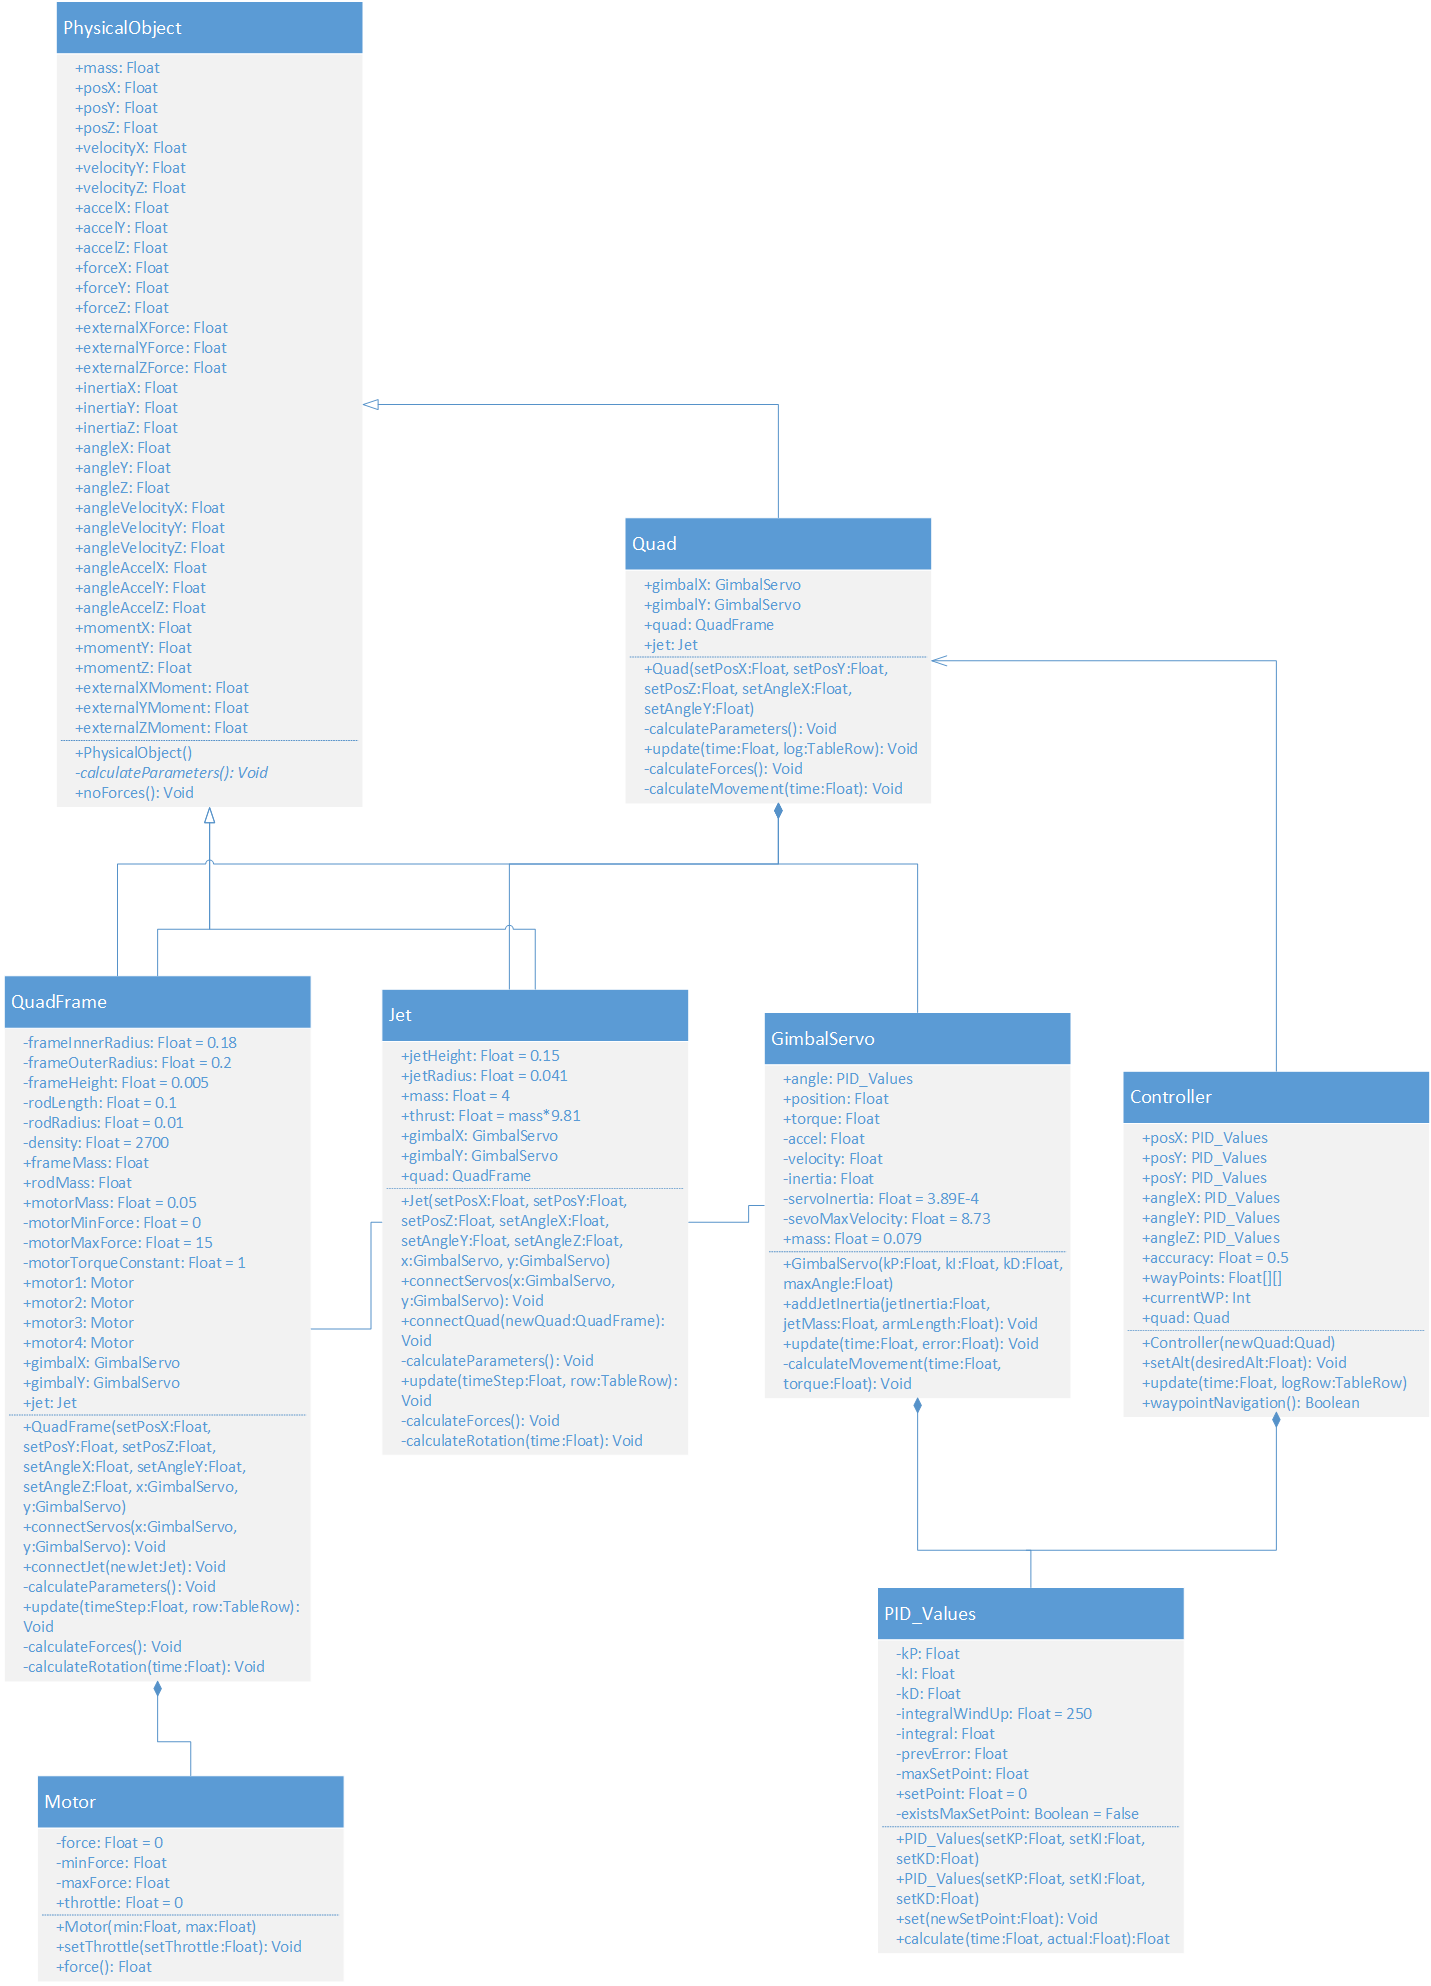
\includegraphics[width=\linewidth]{XQuad_2_Class_Diagram}
    \caption{XQuad2 UML Class Diagram}
    \label{fig:XQuad_2_Class_Diagram}
\end{figure}

It can be seen that there exists a \lstinline|PhysicalObject| class, from which several other classes inherit, which contains attributes which cover information such as mass, position, velocity, and inertia. \lstinline|Quad| contains \lstinline|QuadFrame|, which itself contains 4 \lstinline|Motors|, as well as \lstinline|Jet| and 2 \lstinline|GimbalServos|. \lstinline|QuadFrame|, \lstinline|Jet|, and \lstinline|GimbalServo| are all interconnected, ensuring that changes to one will be accurately and correctly reflected in the other as required.

\lstinline|PID_Values| is a class which describes one set of PID values and the relevant PID calculations, and is used by the \lstinline|GimbalServos| and the \lstinline|Controller|. As described in Section \ref{sec:PID_Control}, standard PID control logic is used, with one addition: integral wind-up has been added. This prevents the integral term from growing disproportionately large, which otherwise occurs in this implementation as our feedback loop occurs several orders of magnitude faster than changes in the output. The code for this is:

\begin{lstlisting}[language=Java]
float calculate(float time, float actual) {
    float error = setPoint - actual;
    integral += (error*time);
    if (integral > integralWindUp) {
        integral = 0;
    }
    float derivative = (error - prevError)/time;
    prevError = error;
    return (kP*error + kI*integral + kD*derivative);
}
\end{lstlisting}

Many classes contain an \lstinline|update()| method. This takes the amount of time that has passed since the last update as an input, and uses this to calculate the resultant movement of the object, as well as recording the result. It uses the current values of velocities and accelerations, as well as exerted forces and moments, by calling methods such as \lstinline|calculateMovement()| and \lstinline|calculateRotation()|.

It should be noted that a minimal effort has been made to make use of object-oriented programming concepts such as encapsulation. The focus of programming this simulation was to produce usable results, not to produce clean, re-usable code.

The full code can be seen in the GitHub repository, located at \url{https://github.com/eugeneval/Project_Titan}.


\subsection{Refinement}
It was realised that the mass of the quad had been implemented incorrectly ($r_r$ had not been squared and the rod mass and motor mass had not been multiplied by 4 in equation \ref{eqn:total_mass}). Additionally, the maximum torque of the servo had not been limited to 0.34kgm. Correcting these resulted in Figures \ref{fig:square_path_limited_servos} and \ref{fig:square_path_limited_servos_angle}.

\begin{figure}
    \begin{subfigure}{\textwidth}
        \includegraphics[width=\linewidth]{square_path_limited_servos}
        \caption{Position}
        \label{fig:square_path_limited_servos}
    \end{subfigure}\hspace*{\fill}
    \\
    \begin{subfigure}{\textwidth}
        \includegraphics[width=\linewidth]{square_path_limited_servos_angle}
        \caption{Angle}
        \label{fig:square_path_limited_servos_angle}
    \end{subfigure}

    \caption{Simulation of a Square Path - With Refinements}
    \label{fig:Square Path Refined}
\end{figure}

These refinements decreased the stability of the drone. It is still well within acceptable parameters for rotation, and for x and y positioning; in fact the steady state error in x and y has been eliminated after further turning of the PID values. The overshoot in height has increased further, and is now over 100\%. There is also a steady state error approximately 1m, and an oscillation also of approximately 1 m.
\label{height overshoot}

\subsection{Conclusion}
The reason for the overshoot in height appears to be that the jet adds mass to the system, without adding weight (as this is cancelled out by its thrust). This is not something that a controller would expect. However, we are not greatly concerned with the accuracy of the height-keeping of the system. As long as we stay above 20ft, the minimum height required by the regulations\cite{IMechE_rules}, it is not a concern.

A simplified model of the airframe configuration has been created and equations of motion derived. A simulation environment has been designed and created from the ground up, and the model created in this simulation. Several configurations have been tested and the results analysed.

It can be seen that the addition of a gimballed jet to a quadcopter does not catastrophically destabilise it. The extremely simple PID controllers used in our simulation are able to cope to a sufficient degree, implying that a significantly more advanced flight stack such as the PX4 should have no problems. Our initial assumption that the jet can simply be ignored is, indeed, valid. We have completed our objectives for this section, as defined in Section \ref{simulation objectives}, determining that the stability of the airframe configuration is within acceptable parameters.



\section{Companion Computer Software: PX4 Control}
\subsection{Introduction}\label{PX4 Control}
We will be controlling the PixHawk flight controller using offboard commands from an external companion computer, henceforth referred to as Pete (since CC is a rather ambiguous acronym). Pete will consist of three main components: communication with the PixHawk, communication with a ground station, and target-finding computer vision.

PixHawk 2 is a fully integrated flight controller running the PX4 flight stack. PX4 is an open source project, and is a further development of the popular ArduPilot flight control software. It is an excellent choice for this project as it is easily adaptable to different vehicles, and is capable of calculating many flight parameters by itself and continuously optimising them. This minimises the amount of work that will be required to adapt it to our custom-built airframe.

PX4 is fully capable of Software-in-the-Loop (SITL) simulation, using either the jMAVSim or Gazebo simulation environments\cite{PX4_dev_guide}. A SITL simulation involves the PX4 software running on a computer and interacting with a physics simulation. This is crucial, as it allows code to be tested with no danger to the real vehicle. Pete can communicate with the simulated vehicle using MAVLink through a UDP port; this is exactly the same as how it would connect to a real vehicle. As far as Pete's code is concerned, there is no difference between a real and a simulated vehicle except for the UDP address.

% Repetition
% Communication with the PX4 flight stack on the PixHawk is based on the DroneKit SDK. This is a platform for devoloping apps written in Python that run on a drone's companion computer. It communicates with the PixHawk using the MAVLink communication protocol.\cite{dronekit} The DroneCore API was also experimented with but proved significantly harder to implement and hence was abandoned.

PX4 has 12 flight modes when employed on a multi-rotor. We are interested in the autonomous modes, which include Hold, Return(RTL), Takeoff, Land, Mission, Follow Me, and Offboard. Of particular interest are Mission, in which `the vehicle follows a programmed mission', and Offboard, where `the vehicle obeys a position, velocity or attitude setpoint provided over MAVLink'\cite{PX4_user_guide}.

The DroneKit SDK was used to create code that will run on Pete and communicate with PX4 using the MAVLink communication protocol. This is an open source, freely available software development kit, specifically designed for offboard control of vehicles using companion computers to enable autonomous behaviour. It is available in three main implementations: on Android, on iOS, and in Python. It is the Python version we will be using here, as almost all available companion computers come with Python preinstalled and with a high level of support for it.

During research into the subject area, two alternative libraries were found that could have been used: MAVROS and DroneCore. These were rejected as they are both written in C++. Although code written in C++ is often faster, it also typically takes longer to write as it is a lower-level language with more need for `boilerplate' code. We did not anticipate our control system to be advanced enough for the speed of code execution to make a significant difference, and developing a control system on time was the larger priority. Python is also more suited to be used as a cross-platform language, which allows for code to be created in one operating system, MacOS, and eventually run in another, specifically Linux (which all available companion computer run on a distribution of).
Additionally, much of the difference can be made up by using C or C++ libraries with Python implementations, as OpenCV, used later in this report, does.

\subsection{Aims and Objectives}
\begin{compactenum}
    \item Research autonomous vehicle flight control solutions and decide on a configuration. \emph{(Already completed)}
    \item Download and set up PX4, JMAVSim, and Dronekit.
    \item Run a SITL PX4 simulation, in conjunction with a jMAVSim simulation, and become familiar with this simulation environment.
    \item Create code using DroneKit that will communicate with the PX4 simulation and JMAVSim.
    \item Create code using DroneKit that will allow for a predetermined flight path to be followed, and test using PX4 and jMAVSim.
    \item Create code using DroneKit that will allows for real-time flight control relative to the current position (required to allow the vehicle to navigate to the target in response to an input from the computer vision module), and test using PX4 and JMAVSim.
    \item Package created code in a module to allow for easy implementation in a full control system.
\end{compactenum}


\subsection{Implementation} \label{control_implementation}
The available documentation and examples for DroneKit mostly make use of the \lstinline|simple_goto()| command\cite{PX4_dev_guide}\cite{dronekit}. Unfortunately, as DroneKit is primarily designed to work with ArduPilot, the predecessor of PX4, this command was discovered to not work when tested in jMAVSim. Neither does \lstinline|arm_and_takeoff()|, or the \lstinline|vehicle.groundspeed| and \lstinline|vehicle.airspeed| attributes, among others.

Additionally, it is usually assumed that one is operating in the \lstinline|global_relative_frame|. There are three frames of reference available:
\begin{center}
\begin{tabular}{cc}
    \lstinline|global_frame| & GPS coordinates, with 0 altitude at sea level \\
    \lstinline|global_relative_frame| & GPS coordinates, with 0 altitude as ground level at the starting location \\
    \lstinline|local_frame| & Cartesian coordinates relative to the starting location
\end{tabular}
\end{center}
\lstinline|local_frame| is the most immediately useful to us, as it is simpler and more intuitive to use. Note that this is the North East Down (NED) frame, i.e. -10m altitude is 10m above the ground.

Custom code has had to be written to take the place of these defunct commands and allow the vehicle to be controlled in the desired manner. First of all, we want to be able to directly send a position waypoint to PX4. This is a feature that is not fully implemented in DroneKit, and so a custom command with a custom MAVLink message has been created:
\begin{lstlisting}[language=Python]
def send_ned_position(pos_x, pos_y, pos_z):

    msg = vehicle.message_factory.set_position_target_local_ned_encode(
        0,       # time_boot_ms (not used)
        0, 0,    # target system, target component
        mavutil.mavlink.MAV_FRAME_LOCAL_NED, # frame
        0b0000111111111000, # type_mask
        pos_x, pos_y, pos_z, # x, y, z positions
        0, 0, 0, # x, y, z velocity in m/s
        0, 0, 0, # x, y, z acceleration (not supported yet)
        0, 0)    # yaw, yaw_rate (not supported yet)

    vehicle.send_mavlink(msg)
\end{lstlisting}

Similarly, other commands have been created to suit our purposes. Some of these have been adapted from examples in the DroneKit and PX4 documentation\cite{PX4_dev_guide}\cite{dronekit}.

\begin{lstlisting}[language=Python]
def arm_and_takeoff(self, targetAlt, accuracy=0.5):
    """Overrides DroneKit command. Takeoff to a target altitude, then loiter."""

    wp = get_location_offset_meters(self.home_location, 0, 0, targetAlt)
    self.commands.add(PX4Command(wp, "TO"))
    self.commands.upload()
    time.sleep(1)

    self.mode = VehicleMode("MISSION")
    time.sleep(1)
    print("Vehicle mode should be MISSION: %s" % self.mode.name)
    self.armed = True
    while True:
        print " Altitude: ", self.location.global_relative_frame.alt
        if self.location.global_relative_frame.alt>=targetAlt-accuracy:
            print "Reached target altitude"
            self.mode = VehicleMode("LOITER")
            time.sleep(0.5)
            break
        time.sleep(1)

def goto_absolute(self, pos_x, pos_y, pos_z, accuracy=0.5, wait=True, text=True):
    """Go to a position relative to the home position"""

    targetLocation = LocationLocal(pos_x, pos_y, -pos_z)

    self.__send_ned_position(pos_x, pos_y, -pos_z)
    self.mode = VehicleMode("OFFBOARD")
    if text: print("Vehicle mode should be OFFBOARD: %s" % self.mode.name)

    while True:
        self.__send_ned_position(pos_x, pos_y, -pos_z)
        remainingDistance = get_distance_metres_local(self.location.local_frame, targetLocation)
        if remainingDistance<=accuracy:
            if text: print("Arrived at target")
            break
        if wait == False: break
        if text: print "Distance to target: ", remainingDistance
        time.sleep(0.1)

def goto_relative(self, pos_x, pos_y, pos_z, accuracy=0.5, wait=True, text=True):
    """Go to a position relative to the current posotion"""

    currentLocation = self.location.local_frame
    targetLocation = get_location_metres_local(currentLocation, pos_x, pos_y, -pos_z)\

    self.__send_ned_position(targetLocation.north, targetLocation.east, targetLocation.down)
    self.mode = VehicleMode("OFFBOARD")
    if text: print("Vehicle mode should be OFFBOARD: %s" % self.mode.name)

    while True:
        self.__send_ned_position(targetLocation.north, targetLocation.east, targetLocation.down)
        remainingDistance = get_distance_metres_local(self.location.local_frame, targetLocation)
        if remainingDistance<=accuracy:
            if text: print("Arrived at target")
            break
        if wait == False: break
        if text: print "Distance to target: ", remainingDistance
        time.sleep(0.1)

def setMaxXYSpeed(self, speed):
    """Required due to DroneKit's vehicle.groundspeed not working with PX4"""

    self.parameters['MPC_XY_VEL_MAX']=speed
    print("Set max speed to: %s" % self.parameters['MPC_XY_VEL_MAX'])
    time.sleep(0.5)

def returnToLand(self):
    """RTL and wait for auto disarm on land"""

    self.mode = VehicleMode("RTL")
    time.sleep(1)
    print("Vehicle mode should be RTL: %s" % self.mode.name)
    while self.armed == True:
        print("Waiting for landing...")
        time.sleep(3)
\end{lstlisting}

\lstinline|arm_and_takeoff()| replaces the command provided in DroneKit, and performs the same function. \lstinline|goto_absolute()| and \lstinline|goto_relative()| allow us to navigate to a position waypoint, simply defined as X meters north, Y meters east, and Z meters up from either the starting location or the current location respectively. The \lstinline|accuracy| attribute optionally allows us to change how close the vehicle must get to the waypoint to consider it to have reached it. \lstinline|setMaxXYSpeed()| is a replacement for the \lstinline|vehicle.groundspeed| attribute present in DroneKit, which does not work as intended with PX4, and allows us to set a maximum groundspeed for the vehicle. Finally, \lstinline|returnToLand()| has the vehicle return to it's starting location and land safely. These commands were all tested using a SITL PX4 simulation in conjunction with jMAVSim.

\subsection{Conclusion}
The code that has been written means that the communication with the PixHawk has been simplified down to a few basic commands. An example mission could consist of the following: arming and taking off, following a series of GPS coordinates, locating a target using computer vision, calculating it's offset from directly underneath the drone, using \lstinline|goto_relative()| to position itself precisely over the target, dropping the payload, returning to base, and landing.

The created code has been throughly tested using a SITL PX4 simulation and jMAVSim, and packaged into a module which can be easily integrated into an overall control system. Using object-oriented programming principles will allow the code to be easily extended or modified later if this is required.


\section{Companion Computer Software: Computer Vision}
The next component of the control system is a computer vision system capable of identifying the target. This takes the form of a red 1x1m square, incorporating an alphanumeric code in white, within a larger 2x2m white square\cite{IMechE_rules}. The system would have to locate the target, calculate the offset from being centered underneath the vehicle, and to identify the alphanumeric code.

Since an interface had already been programmed in Python, it was decided to program the computer vision in Python as well to allow for them to easily work in conjunction. To this end the OpenCV-Python library was chosen.

\subsection{Aims and Objectives}
\begin{compactenum}
    \item Research computer vision solutions and decide on a configuration. \emph{(Already completed)}
    \item Download and compile OpenCV-Python and other relevant packages, and become familiar with them.
    \item Create code that can recognise the IMechE target using computer vision, and test it.
    \item Create code that can read the alphanumeric code inside the IMechE target, and test it.
    \item Create code that can calculate the offset of the target from directly underneath the vehicle (we will use this offset as an input for navigation), and test it.
    \item Package created code in a module to allow for easy implementation in a full control system.
    \item Integrate this new module with the existing control module, and test it using PX4 and jMAVSim.
\end{compactenum}

\subsection{Square Detection}
\begin{wrapfigure}{r}{0.5\textwidth}
    \begin{center}
        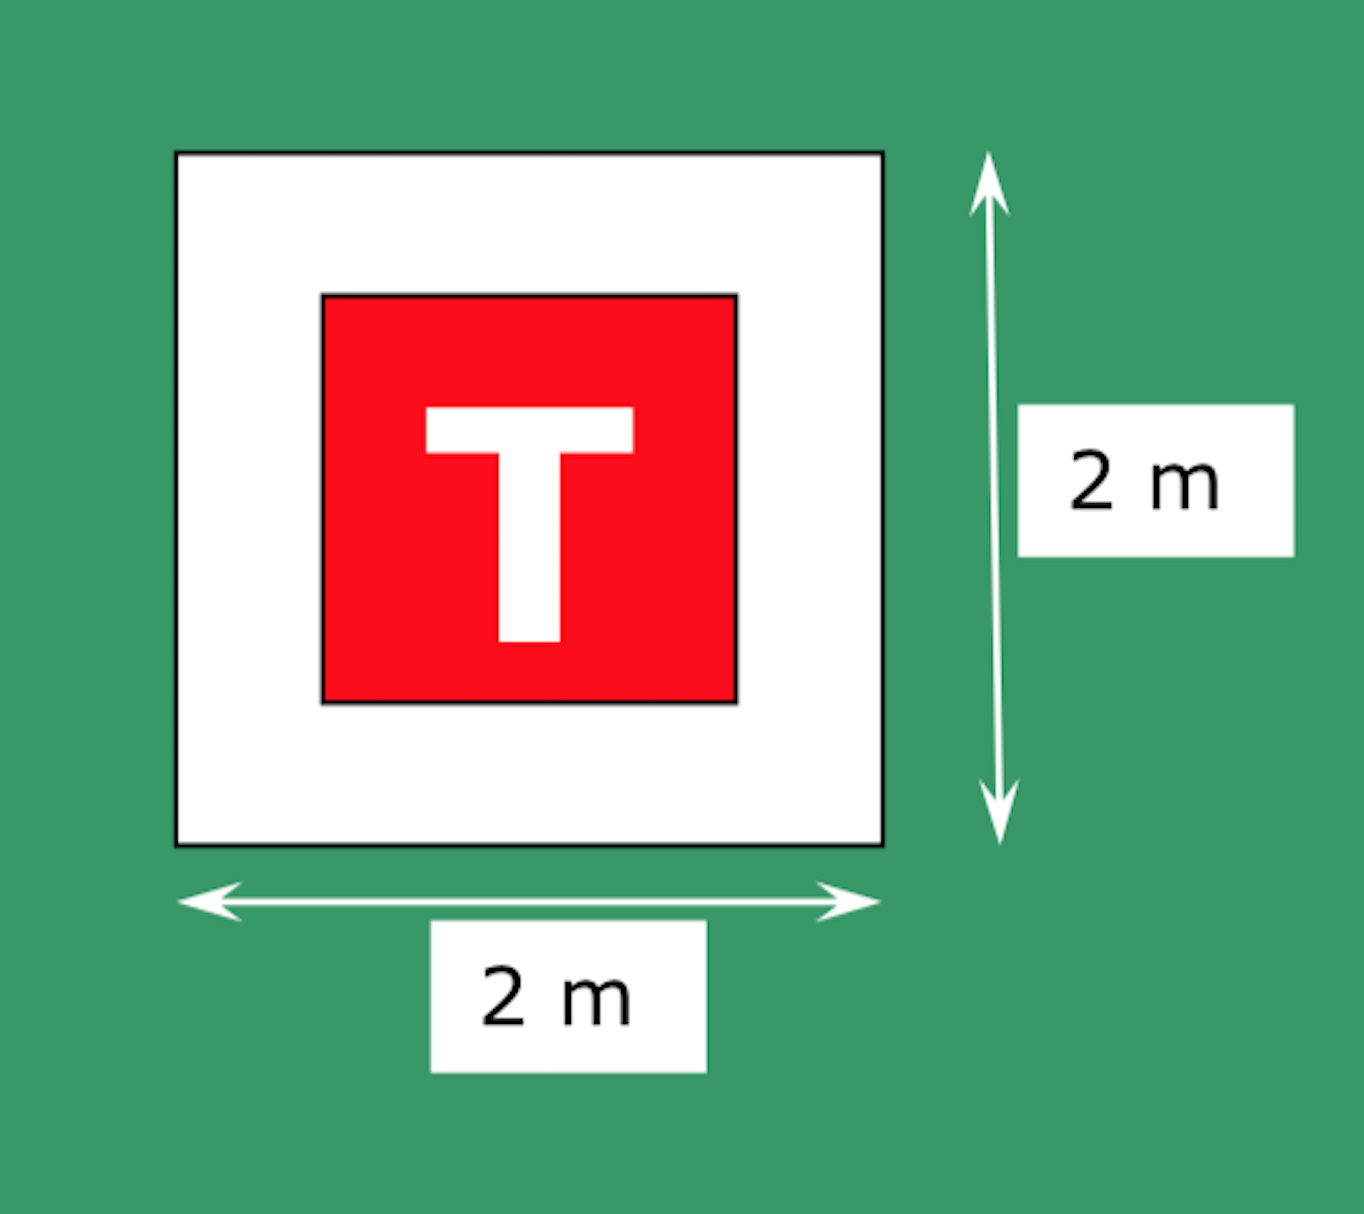
\includegraphics[width=0.48\linewidth]{IMechE_target}
        \caption{Target}
        \label{fig:target}
    \end{center}
\end{wrapfigure}

The target consists of two concentric squares and a central letter, as seen on Figure \ref{fig:target}\cite{IMechE_rules}. Therefore, a good way of identifying the target is looking for concentric squares. This is called feature detection. The other main method is known as creating a cascade, and allows objects whose features cannot be easily described mathematically, such as a chair, to be recognised. However, creating a cascade requires the processing of thousands of images and considerable time. As we are fortunate enough to have a feature which can be described easily mathematically (concentric squares), feature detection is the optimal method.

First, squares are recognised. This is a multi-stage process:
\begin{compactenum}
    \item Convert image to grayscale
    \item Use a Gaussian Blur on the image
    \item Use Canny Edge Detection to find edges
    \item Find complete contours
    \item Find contours that have between 4 and 6 edges
    \begin{compactitem}
        \item An ideal square would have 4 edges, but images are rarely perfect.
    \end{compactitem}
    \item Check that the contour is above a minimum size
    \item Check that the solidity of the contour is above a threshold
    \begin{compactitem}
        \item This is done by drawing a rectangle (the \emph{bounding rectangle}) that encloses the entire contour, and comparing the area of the rectangle to the area of the contour
        \item An ideal square would have a solidity of 1
    \end{compactitem}
    \item Check that the aspect ratio of the bounding rectangle is within thresholds
    \item Contours that have passed all of these criteria must be squares
\end{compactenum}
These contours are then drawn onto the image, showing us the squares. This method can be applied to images, or to video by applying it to each frame in the video. It is modified from examples available online\cite{opencv_tutorials}\cite{pyimagesearch_squares}.

\subsection{Optical Character Recognition}
Reading the letter inside the target is also a requirement of our system. To this end, Optical Character Recognition (OCR) was added to our system. This is done using the freely available Tesseract OCR library, in conjunction with the pytesseract library that adapts it to Python. A simple function was created that takes an image and puts it through Tesseract, printing all that is written on that page. Once again, it was adapted from examples available online\cite{pyimagesearch_ocr}.

It should be noted that the function which performs this OCR was discovered to be extremely inefficient, taking about 0.3 seconds to execute, due to the way that the Tesseract library is accessed. This would decrease the frame rate below usable levels if run routinely, and so will only be run a single time once the target has been positively identified.

\subsection{Target Detection}
The next step was to find the target by finding squares that are concentric to each other. This was done by finding the coordinates of the center of the square, using OpenCV's \lstinline|moments()| function. This center was then compared to the centers of all other squares that had been found.

At this point, a \lstinline|Square| class was made to improve the code under the concepts of object-oriented programming. A \lstinline|concentric()| method was made in this class that compares squares against each other to see if their center points are within a certain distance of each other (by default, 5\% of the size of the square). Two squares that are concentric are added to a new instance of a \lstinline|Target| class. Repeated comparisons are avoided by using \lstinline|intertools.combinations()| to make a list of all the unique pairs of squares before comparing.

Initially, it appeared that all squares were targets. The problem was discovered to be that there were in fact multiple, very similar squares being generated for each actual square on the image. For example, for a square whose border is a black line might have the outside of the line and the inside of the line counted as separate squares. These squares are clearly concentric and thus all squares are targets. The problem was solved by creating a \lstinline|similar()| method for \lstinline|Square| and using it to eliminate squares that are too similar (again, 5\% by default), ensuring that all squares are unique before running the \lstinline|concentric()| method to find targets.

From here, it is trivial to calculate the offset of the target from the center of the image or camera frame. This offset will be used as an input into a control system to move the drone above the target.

\subsection{Integrating into Control}
Using the code developed in Section \ref{control_implementation}, a program was created to integrate the newly-developed computer vision. This takes off to 10m, and once there the webcam on the computer is turned on. It looks for a target, and uses the offset of the target from the center of the camera as an input for the desired position of the drone. This was verified to work as intended, validating all the work we have done up to this point.

Multithreading was used to optimise performance and increase effectiveness. Unfortunately, it could not be fully implemented, as OpenCV's \lstinline|VideoCapture()|, used to receive input from the camera, is only capable of functioning inside the main thread. This is a known unresolved issue with OpenCV itself. This meant that receiving input could not occur in a subthread, which is unfortunate as input/output operations are normally the most desirable operation to keep in subthreads. In this version of the program, the main thread handles computer vision and a subthread contains the \lstinline|vehicle| class which communicates with the PixHawk. \label{OpenCV_multithreading_issues}

A demonstration video of this was created. For obvious reasons, it could not be put in this report, but is available at \url{https://youtu.be/sFyZphH8_CM}.

\subsection{Investigating Frame Rate}
The method of finding all squares, checking through them all for duplicates, then checking through them all for targets, intuitively seems inefficient. This could especially become an issue when deployed to a drone platform, which will likely have less processing power.

However, timing sections of the program using the \lstinline|timeit| library revealed that the vast majority of the time that went into processing a frame went into receiving a frame from the camera, with the entire process of target detection taking approximately 10\% of the required time per frame. This is because I/O (Input/Output) operations are very expensive in terms of computing time. Meanwhile all the square comparisons are simple number comparisons, which are cheap.

Thus, it was decided there was no need to optimise the target-finding algorithm, as it would have a minimal effect on frame rate. Any appreciable frame rate improvement will have to come from improving the speed of obtaining a frame from the camera.

\subsection{Conclusion}
A module has been created, throughly tested, and integrated that allows for IMechE targets to be recognised and used to navigate the vehicle.

Investigations have been made into multithreading and frame rate. These can be taken further once a specific companion computer is chosen, as any improvements that can be made here are heavily dependent on the specific architecture of the chosen computer and operating system.

Potentially, some of the parameters used to identify the target will need to be fine-tuned once deployed on a real vehicle to account for how the target may look different. The code has been written in such a way that these parameters are easy to modify.

\section{Companion Computer Software: Communication}
Communication from Pete, our companion computer, to a base station to transmit information will, by necessity, be over a serial connection, as this is how most low-end radio links are designed.

The socat command line utility was used to establish two virtual serial ports which communicate with each other. These are then accessed using the pyserial library to write and read information from these serial ports.

\subsection{Aims and Objectives}
\begin{compactenum}
    \item Research serial communication solutions and decided on a configuration. \emph{(Already completed)}
    \item Download and become familiar with relevant libraries.
    \item Create code that will allow for relevant information to be sent over a serial connection, and test it using socat.
    \item Package created code in a module to allow for easy implementation in a full control system.
    \item Integrate this new module with existing software, and test it.
\end{compactenum}


\subsection{Implementation}
Several methods for serialising information was investigated. Python has a library called \lstinline|pickle|, which converts an object to a serial format by `pickling' it, and `unpickling' into the complete object at the other end of the serial connection. This method was investigated, but has certain limitation with the types of data that can be pickled and unpickled, and is also somewhat unreliable.

Instead, the JavaScript Object Notation (JSON) was used. This is a standard method of formatting the attributes of objects to a text string, which can then be sent over a serial connection. JSON is a well established method for transmitting object attributes over many different kinds of connections between different devices and programming languages, and is a good solution as it is inherently simple and reliable.

It was quickly discovered that sending an entire image over a serial connection within a reasonable amount of time is not possible. Even sending the contours of a square does not work well, as this is a large set of points. Thus, it was decided to send only the most important information.

A \lstinline|Square2| and \lstinline|Target2| class were created. These inherit from \lstinline|Square| and \lstinline|Target|. The only difference is that they are missing the contours of the squares. \lstinline|Square| and \lstinline|Target| gained a \lstinline|to_json()| method that converts their attributes to a string using JavaScript Object Notation (JSON), a standard for transmitting information. \lstinline|Square2| and \lstinline|Target2| have a function \lstinline|from_json()| which can recreate the squares from the JSON string.

This was tested by sending the targets over the virtual serial connection, and drawing them on the image. With minor modifications to the way that squares and targets are drawn, this worked successfully. Notably, squares are now defined largely based on their bounding rectangle and not on their own contours, which for a square or rectangle makes little difference.

\subsection{Conclusion}
Through the usage of JSON and the pyserial library the location of a target can be sent over a serial connection. This has been tested using socat and integrated into existing functionality.

The UAS Challenge requires the GPS coordinates of a target to be relayed to the base station. This will be done by knowing the current location of the vehicle using our control module, and knowing the offset of the target from directly underneath the vehicle. Calibration will be needed upon deployment on a real vehicle to ensure accuracy, but otherwise this module is complete.

\section{Companion Computer Software: Other Concerns}
\subsection{Jet Engine Control \& Payload Delivery}
The thrust output of the MJE will need to be controlled to compensate for the change in weight as payloads are dropped. Additionally, by more closely controlling jet thrust it may be possibly to reduce the instability in height noted in Section \ref{height overshoot}.

The MJE is controlled with a FADEC that takes a PWM (Pulse Width Modulation) signal as an input. PWM is a standard method of sending a digital signal to control a single variable such as speed on a motor, widely used in electronics; most companion computers are capable of creating such a signal using output pins and libraries for it in Python are widely available. This input signal can vary from 1000 to 2000 microseconds, and the FADEC is fully configurable as to what this range represents. In our case, it has been configured so that 1000 microseconds corresponds to idle and 2000 microseconds corresponds to maximum thrust.

\begin{wrapfigure}{r}{0.5\textwidth}
    \begin{center}
        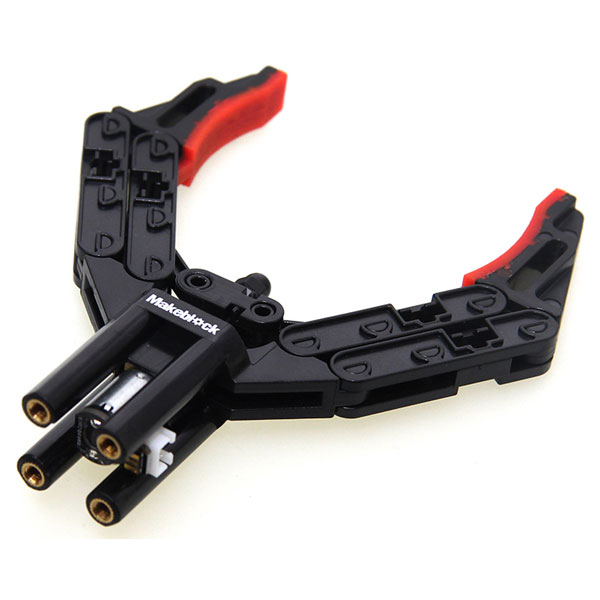
\includegraphics[width=0.48\linewidth]{makeblock_gripper}
        \caption{Makeblock 86502 Robot Gripper}
        \label{fig:makeblock_gripper}
    \end{center}
\end{wrapfigure}

Additionally, a mechanism to control the payload delivery mechanism is also required. Development of the specifics of payload delivery is being undertaken by a 1st year student, Arkadiy Serezhkin. The current solution will likely use a servo mechanism of some description. An example of such a mechanism would be the Makeblock 86502 Robot Gripper\cite{Makeblock_gripper}, seen in Figure \ref{fig:makeblock_gripper}.

The issue of a moving center of gravity when a payload is dropped is also an issue that is currently being investigated. Placing the payload underneath the jet engine, with a cone to divert the jet exhaust, was rejected due to the large loss of thrust from the jet this would cause. Placing the payloads evenly distributed, as close to the center of the vehicle as possible, still raises issues with one of the electric motors having to take on too much of the weight. Whatever the final solution, it may well factor in to the programming required for the payload drop mechanism. \label{payload_delivery}

The full implementation of this will depend on the specific companion computer chosen, as the libraries to output signals using the output pins of a companion computer are specific to that companion computer, as well as the final payload deliver method chosen. For now, a \lstinline|Payload| class has been created, and incorporated into the \lstinline|Vehicle|. Later, the specific code for controlling payload drops, and varying jet engine thrust in response to payload drops, will be incorporated into this class.

\subsection{Choosing a Computer} \label{cc_selection}
By this point, Pete has advanced about as far as is possible in a purely simulated environment. Further development required moving onto a real companion computer, and testing either with a real drone or a Hardware-in-the-Loop (HITL) simulation.

A comparison was made of available companion computers on the market. The Intel Edison, Raspberry Pi3, Nvidia TX2, Odroid XU4, and Snapdragon Flight were compared on criteria such as processing power, weight, and cost. The full comparison can be seen in Figure \ref{fig:cc_selection}.

\begin{figure}[h]
    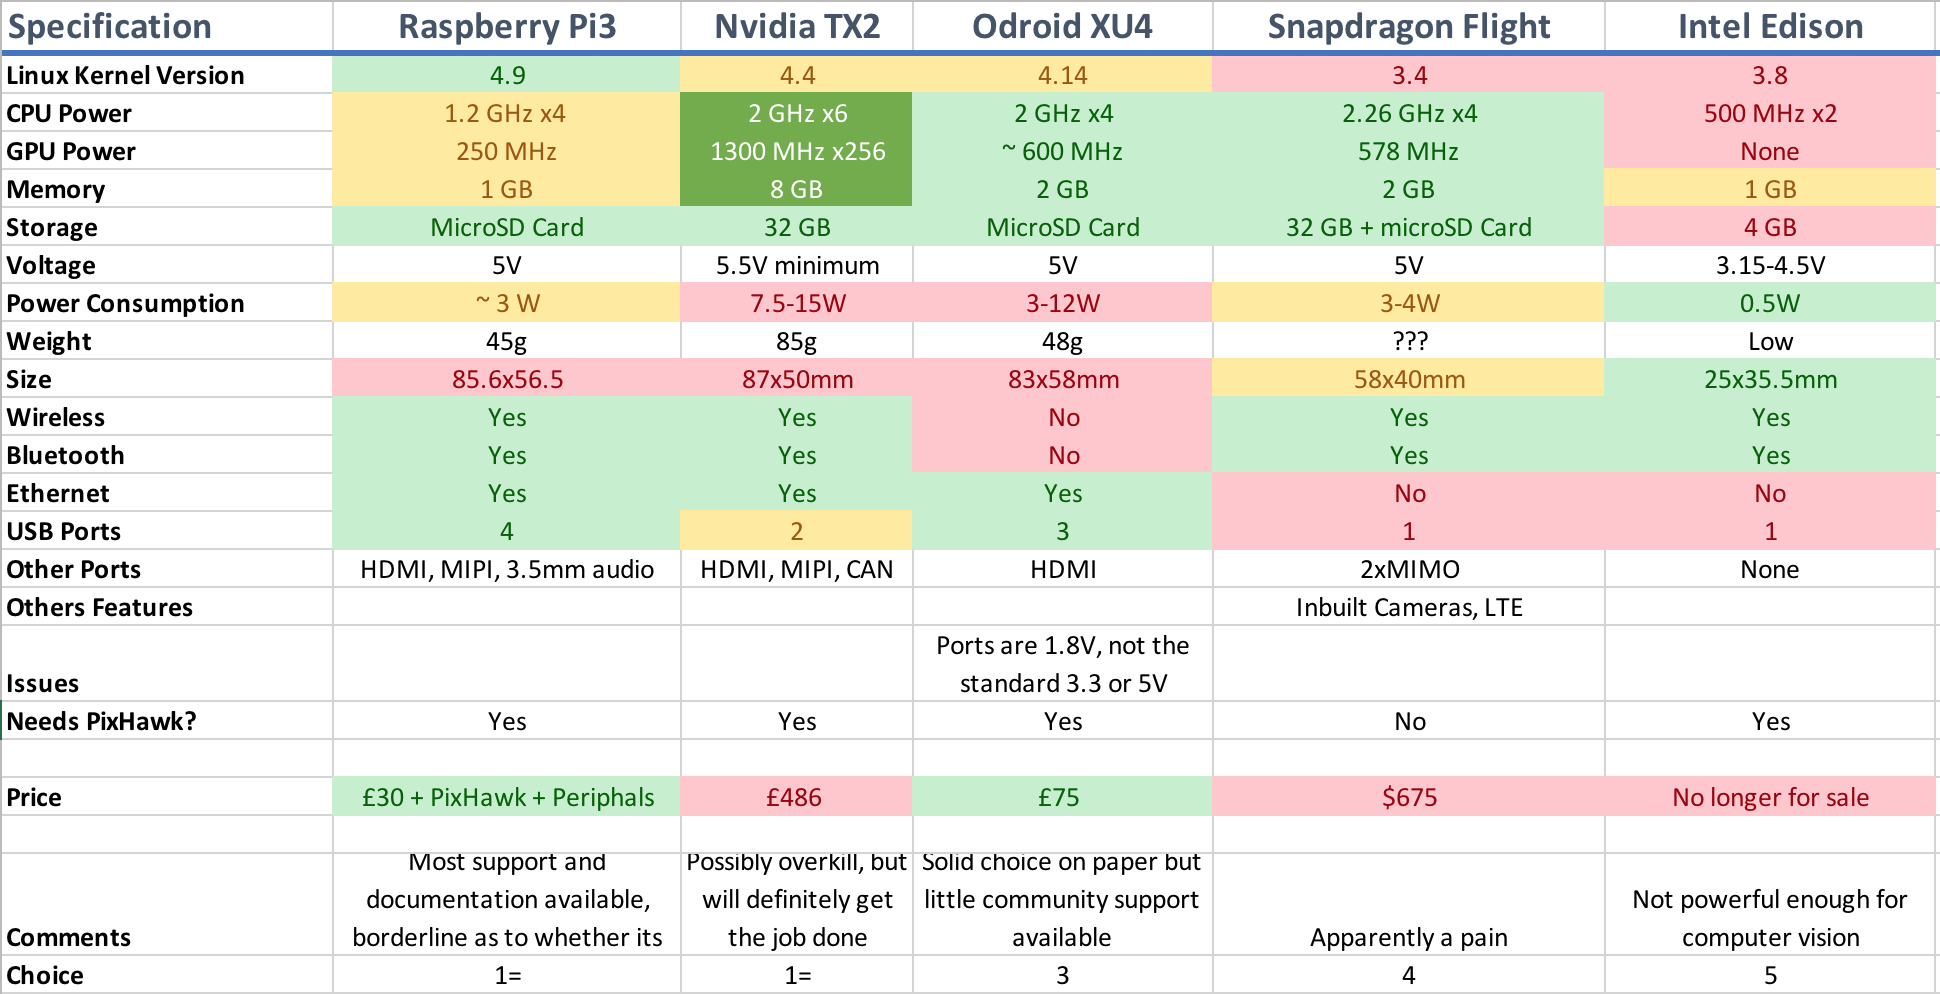
\includegraphics[width=\linewidth]{companion_computer_comparison}
    \caption{Companion Computer Selection} \label{fig:cc_selection}
\end{figure}

Of these, the Raspberry Pi3 was the preferred choice, as it is cheap and light, and has the greatest amount of community support and available documentation. It is, however, borderline as to whether it is powerful to run the required computer vision computation\cite{companion_computer_power}. The Nvidia TX2 is a close second. It is definitely powerful enough to meet our needs, but is significantly more expensive and has less support available. It was therefore decided to buy a Raspberry Pi, and to upgrade to the TX2 if it turns out to not be powerful enough.


\subsection{Companion Computer Setup \& Testing}
A Raspberry Pi3, along with camera, was obtained, and Raspbian (a distribution of Linux specifically designed for the Pi) was installed on it. There were some initial problems with insufficient memory space, as OpenCV requires approximately 4GB of free space to compile. After the installation of a larger memory card, OpenCV was successfully compiled, and other required libraries such as DroneKit were also acquired.

Slight modification to the existing code needed to made, mainly that the \lstinline|picamera| library was used as an intermediary between the Pi's camera and the existing computer vision code.

When tested the code performed as expected, communicating with the simulation running on the main computer over a UDP connection, and recognising targets using the Pi's camera. This is important because it means the companion computer is ready to be installed on the vehicle, and also validates the choice of Python as a cross-platform programming language.

\section{Conclusion \& Further Work}
\begin{compactenum}
    \item The stability of the airframe configuration has been examined in a simulated environment, and shown to be within acceptable parameters in the x and y directions. There is a large overshoot and not inconsiderable oscillation in z (height), but this is acceptable as the required precision in height for our vehicle is very low.
    \item A control system has been designed and tested within a simulated environment, which can:
    \begin{compactenum}
        \item Travel to predetermined GPS waypoints.
        \item Recognise and navigate to a target using computer vision.
        \item Communicate the GPS coordinate of the target to a ground station.
    \end{compactenum}
    \item The control system has been uploaded to and adapted for a companion computer.
\end{compactenum}
\vspace{1em}

More detail on each of these completed objectives is available within the sub-conclusions seen throughout the report. The stability of the system was examined by creating a model and simulation from scratch in Processing. The computer companion code has been tested using a SITL PX4 simulation in conjunction with jMAVSim, as well as individual Python unit tests where appropriate.

The control system has been tested as far as is possible within the current simulated environment. The next stage is preferably deployment on a real platform, where further testing and development can take place. This is dependent on Ismail delivering a working airframe; at the time of writing, all design work has been completed with manufacturing to commence shortly\cite{Ismail_paper}.

An alternative would be to move to a more advanced simulation environment, specifically Gazebo, which is an advanced robotics and physics simulation library and which is capable of interfacing with a PX4 simulation\cite{PX4_dev_guide}. Enough research and investigation has been done into this to discover that creating an accurate simulation in Gazebo, with our custom airframe modelled correctly and integrated with the PX4 simulation, is almost ambitious enough to form a third-year project in and of itself.

The design of the control system so far allows for a great deal of flexibility and expansion through the use of object-oriented programming, although further work could be done in this area, especially when it comes to the usage of OpenCV and multithreading (This is a known issue, as described in Section \ref{OpenCV_multithreading_issues}). The use of the \lstinline|picamera| module rather than OpenCV's \lstinline|VideoCapture| may allow image processing to be moved into a subthread and proper multithreading implemented. Additionally, the code that has been written could be better packaged, although this would only really become an issue if it was being distributed.

The successful manufacture and testing of a drone platform using this airframe configuration would open the door for further development. Due to the use of the MJE the configuration inherently has a high power to weight ratio, and scales up to larger sizes very well\cite{Ismail_paper}. The validation of this vehicle concept could lead to a new generation of unmanned aerial systems.




%%%%%%%%%%%%%%%%%%%%%%%%%%%%%%%%%%%%%%%%%%%%%%%%%%%%%%%%%%%%%%%%%%%%%%%%%%%%%%%
% APPENDIX
%%%%%%%%%%%%%%%%%%%%%%%%%%%%%%%%%%%%%%%%%%%%%%%%%%%%%%%%%%%%%%%%%%%%%%%%%%%%%%%
\newpage
\appendix
\section{Table of All Symbol Definitions}
\begin{center}
    \emph{Note: values are only given for variables which are constants. No values are given for values derived from constants or for dynamic variables.}
\begin{longtable}{|ccc|}
    \hline
    \emph{Symbol} & \emph{Definition} & \emph{Value(where appropriate)} \\
    \hline \endhead
    & \emph{Positions and Angles} & \\
    \hline
    $\theta_x$ & Quad Pitch & \\
    $\theta_y$ & Quad Roll & \\
    $\theta_z$ & Quad Yaw & \\
    $\phi_x$ & Jet Pitch & \\
    $\phi_y$ & Jet Roll & \\
    $\phi_z$ & Jet Yaw & \\
    \hline
    & \emph{Dimensions} & \\
    \hline
    $h_f$ & Quad frame height & 5 mm \\
    $r_1$ & Quad frame inner radius & 180 mm \\
    $r_2$ & Quad frame outer radius & 200 mm \\
    $L_R$ & Quad arm length & 100 mm \\
    $r_r$ & Quad arm radius & 2 mm \\
    $r_J$ & Jet radius & 41 mm \\
    $h_J$ & Jet height & 150 mm \\
    $l_c$ & Gimbal servo connecting rod length & 100 mm \\
    \hline
    & \emph{Masses} & \\
    \hline
    $M_{TOT}$ & Total Mass & \\
    $\rho$ & Density of Quad & $2700 kgm^3$ \\
    $M_F$ & Quad frame mass & \\
    $M_R$ & Quad rod mass & \\
    $M_M$ & Motor mass & 50 g \\
    $M_G$ & Gimbal servo mass & 79 g \\
    $M_J$ & Jet mass & 4 kg\\
    \hline
    & \emph{Inertias} & \\
    \hline
    $I_{Qx}$ & Quad inertia about x axis & \\
    $I_{Qy}$ & Quad inertia about y axis & \\
    $I_{Qz}$ & Quad inertia about z axis & \\
    $I_{Jx}$ & Jet inertia about x axis & \\
    $I_{Jy}$ & Jet inertia about y axis & \\
    $I_{Jz}$ & Jet inertia about z axis & \\
    \hline
    & \emph{Forces} & \\
    \hline
    $F_x$ & Sum of forces in x direction & \\
    $F_y$ & Sum of forces in y direction & \\
    $F_z$ & Sum of forces in z direction & \\
    $F_{M1}$ & Force from motor 1 & \\
    $F_{M2}$ & Force from motor 2 & \\
    $F_{M3}$ & Force from motor 3 & \\
    $F_{M4}$ & Force from motor 4 & \\
    $F_J$ & Force from jet & \\
    \hline
    & \emph{Torques and Moments} & \\
    \hline
    $\tau_{Qx}$ & Sum of moments on quad about x axis & \\
    $\tau_{Qy}$ & Sum of moments on quad about y axis & \\
    $\tau_{Qz}$ & Sum of moments on quad about z axis & \\
    $\tau_{Gx}$ & Torque of jet gimbal servo about x axis & \\
    $\tau_{Gy}$ & Torque of jet gimbal servo about y axis & \\
    \hline
    & \emph{PID Controllers} & \\
    \hline
    $SP_x$ & Quad X position controller setpoint & \\
    $SP_y$ & Quad Y position controller setpoint & \\
    $SP_z$ & Quad Z position controller setpoint & \\
    $SP_{\theta_x}$ & Quad X angle controller setpoint & \\
    $SP_{\theta_y}$ & Quad Y angle controller setpoint & \\
    $SP_{\theta_z}$ & Quad Z angle controller setpoint & \\
    $O_x$ & Quad X position controller output & \\
    $O_y$ & Quad Y position controller output & \\
    $O_z$ & Quad Z position controller output & \\
    $O_{\theta_x}$ & Quad X angle controller output & \\
    $O_{\theta_y}$ & Quad Y angle controller output & \\
    $O_{\theta_z}$ & Quad Z angle controller output & \\
    $SP_{\phi_x}$ & Jet X angle controller setpoint & \\
    $SP_{\phi_y}$ & Jet Y angle controller setpoint & \\
    $O_{\phi_x}$ & Jet X angle controller output & \\
    $O_{\phi_y}$ & Jet Y angle controller output & \\
    \hline
\end{longtable}
\end{center}

\newpage
\section{Table of Abbreviations}
\begin{center}
    In alphabetical order:
    \begin{longtable}{|cc|}
        \hline
        \emph{Abbreviation} & \emph{Definition} \\
        \hline \endhead
        API & Application Programming Interface \\
        APM & ArduPilot Mega \\
        ESC & Electronic Speed Control \\
        FADEC & Full Authority Digital Engine Control \\
        GPS & Global Positioning System \\
        HITL & Hardware In The Loop \\
        I/O & Input/Output \\
        IMechE & Institution of Mechanical Engineers \\
        JSON & JavaScript Object Notation \\
        MAVLink & Micro Air Vehicle Link \\
        MAVROS & Micro Air Vehicle Robotic Operating System \\
        MJE & Micro Jet Engine \\
        NED & North East Down \\
        OCR & Optical Character Recognition \\
        PID & Proportional Integral Derivative \\
        PWM & Pulse Width Modulation \\
        PWM & Pulse Width Modulation \\
        RTL & Return To Land \\
        SDK & Software Development Kit \\
        SITL & Software In The Loop \\
        UAS & Unmanned Aerial Systems \\
        UDP & User Datagram Protocol \\
        UML & Unified Modelling Language \\
        \hline
    \end{longtable}
\end{center}



%%%%%%%%%%%%%%%%%%%%%%%%%%%%%%%%%%%%%%%%%%%%%%%%%%%%%%%%%%%%%%%%%%%%%%%%%%%%%%%
% BIBLIOGRAPHY
%%%%%%%%%%%%%%%%%%%%%%%%%%%%%%%%%%%%%%%%%%%%%%%%%%%%%%%%%%%%%%%%%%%%%%%%%%%%%%%
\newpage
\small
\begin{thebibliography}{11}

\bibitem{IMechE_about_uas}
    IMechE. About UAS Challenge - IMechE [Internet]. [Accessed 20 December 2017]; Available from: \url{https://www.imeche.org/events/challenges/uas-challenge/about-uas-challenge}.

\bibitem{IMechE_rules}
    Institution of Mechanical Engineers. University UAS Challenge 2018 Competition Rules [Internet]. Issue 7.1. [Accessed 27 December 2017]; Available from: \url{https://www.imeche.org/docs/default-source/1-oscar/uas-challenge/uas-challenge--competition-rules.pdf?sfvrsn=2}.

\bibitem{PX4_user_guide}
    DroneCode. PX4 Autopilot User Guide [Internet]. Updated 20 December 2017. [Last accessed 20 December 2017]; Available from: \url{https://docs.px4.io/en/}.

\bibitem{PX4_dev_guide}
    DroneCode. PX4 Development Guide [Internet]. Updated 15 December 2017. [Last accessed 20 December 2017]; Availible from: \url{https://dev.px4.io/en/}.

\bibitem{dronekit}
    3D Robotics. DroneKit-Python Documentation [Internet]. Updated 21 April 2017. [Accessed 20 December 2017]; Available from: \url{http://python.dronekit.io}.

\bibitem{opencv_tutorials}
    OpenCV. OpenCV-Python Tutorials — OpenCV 3.0.0-dev documentation [Internet]. Last updated 10 Novemeber 2014. [Accessed 22 December 2017]; Available from: \url{https://docs.opencv.org/3.0-beta/doc/py_tutorials/py_tutorials.html}.

\bibitem{pyimagesearch_squares}
    Adrian Rosebrock. Target acquired: Finding targets in drone and quadcopter video streams using Python and OpenCV [Internet]. 4 May 2015. [Accessed 22 December 2017]; Available from: \url{https://www.pyimagesearch.com/2015/05/04/target-acquired-finding-targets-in-drone-and-quadcopter-video-streams-using-python-and-opencv/}.

\bibitem{pyimagesearch_ocr}
    Adrian Rosebrock. Using Tesseract OCR with Python [Internet]. 10 July 2017. [Accessed 22 December 2017]; Available from: \url{https://www.pyimagesearch.com/2017/07/10/using-tesseract-ocr-python/}.

\bibitem{Makeblock_gripper}
    Rapid Eletronics Limited. Makeblock 86502 Robot Gripper up to 1.5KG with 12V Motor [Internet]. [Accessed 16 April 2018]; Available from: \url{https://www.rapidonline.com/Makeblock-86502-Robot-Gripper-up-to-1-5KG-with-12V-Motor-75-0703?IncVat=1&pdg=aud-313476734810:pla-339342696145:kwd-339342696145:cmp-757438067:adg-44804851896:crv-207912323492:pid-75-0703:dev-c&gclid=CjwKCAjwk9HWBRApEiwA6mKWaUnklYF9qNoe1kG8G0wc0quum8lmKrSm6ndSPCsK9-yZVVFx949oThoCedMQAvD_BwE}

\bibitem{companion_computer_power}
    Dries Hulens, Jon Verbeke and Toon Goedem\'e. How to choose the best embedded processing platform for on-board UAV image processing. In: Computer Vision, Imaging and Computer Graphics Theory and Applications edition:VISIGRAPP 2015 pages:455-472.

\bibitem{quad_modelling_matlab}
    Fernando HC, De Silva AT, De Zoysa MD, Dilshan KA, Munasinghe SR. Modelling, simulation and implementation of a quadrotor UAV. InIndustrial and Information Systems (ICIIS), 2013 8th IEEE International Conference on 2013 Dec 17 (pp. 207-212). IEEE.

\bibitem{quadcopter_dynamics}
    Andrew Gibiansky. Quadcopter Dynamics, Simulation, and Control [Internet]. 23rd Nov 2012. [Accessed 23 November]; Available from: \url{http://andrew.gibiansky.com/downloads/pdf/Quadcopter%20Dynamics,%20Simulation,%20and%20Control.pdf}

\bibitem{student_drone_platform}
    Mathias HD. An autonomous drone platform for student research projects. Journal of Computing Sciences in Colleges. 2016 May 1;31(5):12-20.

\bibitem{quad_modelling}
    Luukkonen T. Modelling and control of quadcopter. Independent research project in applied mathematics, Espoo. 2011 Aug 22;22.

\bibitem{PID_tuning}
    Leong BT, Low SM, Ooi MP. Low-cost microcontroller-based hover control design of a quadcopter. Procedia Engineering. 2012 Jan 1;41:458-64.

\bibitem{Ismail_paper}
    Syed Ismail Ahamad. Unmanned Ariel Systems. MECH3002 Final Report. 25 April 2018.

\bibitem{processing}
    Processing 3. Processing Foundation. \url{https://processing.org}.

\bibitem{python}
    Python 2.7. Python Software Foundation. \url{https://www.python.org/}.

\bibitem{socat}
    socat - Multipurpose relay (SOcket CAT). Gerhard Rieger. \url{http://www.dest-unreach.org/socat/doc/socat.html#CREDITS}.

\end{thebibliography}

\end{document}
